\documentclass[12pt]{amsart}
\usepackage{float}
\usepackage[margin=1.1in]{geometry}
\usepackage{graphicx}
\linespread{1.0}
\newcommand{\ZZ}{\mathbb{Z}}
\newcommand{\QQ}{\mathbb{Q}}
\newcommand{\RR}{\mathbb{R}}
\newcommand{\CC}{\mathbb{C}}
\newcommand{\HH}{\mathbb{H}}
\newcommand{\FF}{\mathbb{F}}

\newcommand{\rank}{\mathop\mathrm{rank}}
\newcommand{\supp}{\mathop\mathrm{supp}}
\newcommand{\tr}{\mathop\mathrm{tr}}
\newcommand{\Span}{\mathop\mathrm{span}}

\newcommand{\cl}[1]{\overline{#1}}
\newcommand{\Id}{\mathop\mathrm{Id}}
\newcommand{\Int}{\mathop\mathrm{int}}

\newcommand{\Exercise}[1]{\ \par\noindent\textbf{\em{[#1]}}\\}
\newcommand{\Subexe}[1]{\ \par\noindent\textbf{\em{(#1).}}~}
\newcommand{\Subsubexe}[1]{\ \par\indent\emph{(#1).}~}

\makeatletter
\renewcommand{\section}{\@startsection{section}{1}{0mm}
{-\baselineskip}{0.5\baselineskip}{\bf\leftline}}
\makeatother

\begin{document}
\noindent CSci 5512 -- Artificial Intelligence II \hfill Jiecao Chen \hfill ID:4716311 \\
\textsc{Homework \#2 \hfill Due: Due Wed, Mar 13}\\

\section*{Question 1} 
\subsection*{a}
$P(C|r,w,s)\\
\indent =\alpha P(C,r,w,s)\\ 
\indent =\alpha P(C)P(r|C)P(s|C)P(w|s,r)\\
\indent =\alpha \langle 0.5,0.5\rangle\langle 0.8,0.2\rangle\langle 0.1,0.5\rangle\times 0.99\\
\indent =\alpha \langle 0.0396,0.0459\rangle\\
\indent =\langle 0.4444,0.5556\rangle$\\

$P(C|\neg r,w,s)\\
\indent =\alpha P(C,\neg r,w,s)\\ 
\indent =\alpha P(C)P(\neg r|C)P(s|C)P(w|s,\neg r)\\
\indent =\alpha \langle 0.5,0.5\rangle\langle 0.2,0.8\rangle\langle 0.1,0.5\rangle\times 0.90\\
\indent =\alpha \langle 0.009,0.18\rangle\\
\indent =\langle 0.047619,0.952381\rangle$\\


$P(R|c,w,s)\\
\indent =\alpha P(c,R,w,s)\\ 
\indent =\alpha P(c)P(R|c)P(s|c)P(w|s,R)\\
\indent =\alpha 0.5\times \langle 0.8,0.2\rangle\times 0.1 \times \langle 0.99,0.90\rangle\\
\indent =\alpha \langle 0.0396, 0.009\rangle\\
\indent =\langle 0.814815, 0.185185\rangle$\\

$P(R|\neg c,w,s)\\
\indent =\alpha P(\neg c,R,w,s)\\ 
\indent =\alpha P(\neg c)P(R|\neg c)P(s|\neg c)P(w|s,R)\\
\indent =\alpha 0.5\times \langle 0.2,0.8\rangle\times 0.5 \times \langle 0.99,0.90\rangle\\
\indent =\alpha \langle 0.0495, 0.18\rangle\\
\indent =\langle 0.215686, 0.784314\rangle$\\
PS: The first part is assigned as \textbf{True} and the second \textbf{False}
\subsection*{b}
Python code has be independently created.\\
One possible output is : $P(r|s,w) = 0.31926$


\section*{Question 2}
\subsection*{a}
See fig 1
\begin{figure}[H]
  \centering
  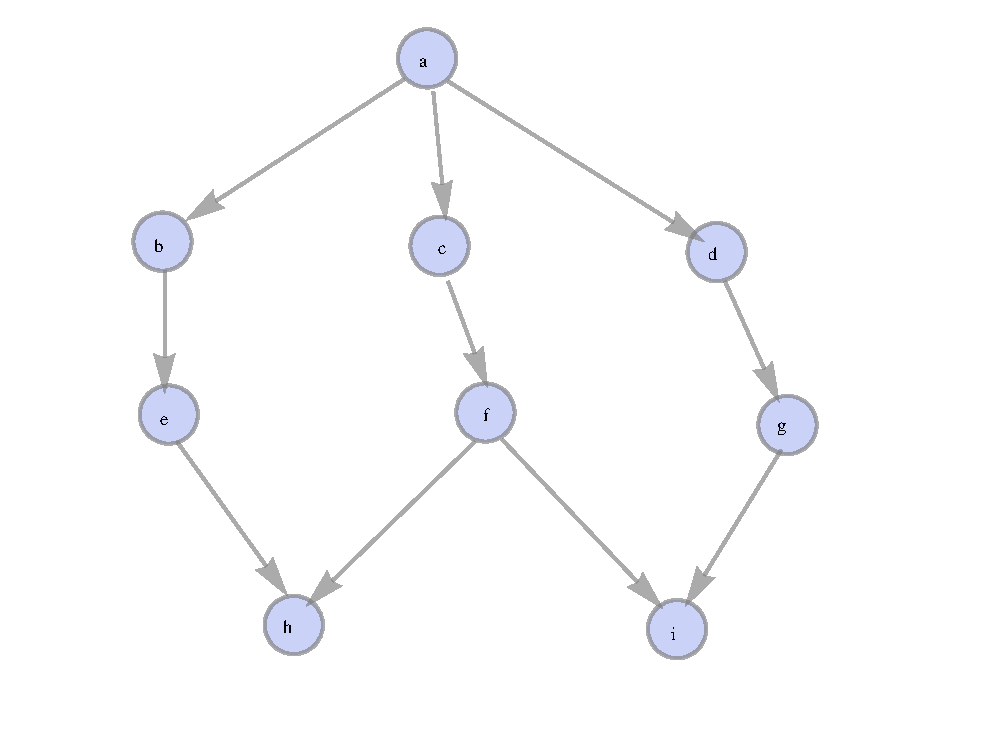
\includegraphics[width=0.8\textwidth]{BN.pdf}
  \caption{Belief Network}
\end{figure}

\subsection*{b}
See fig 2
\begin{figure}[H]
  \centering
  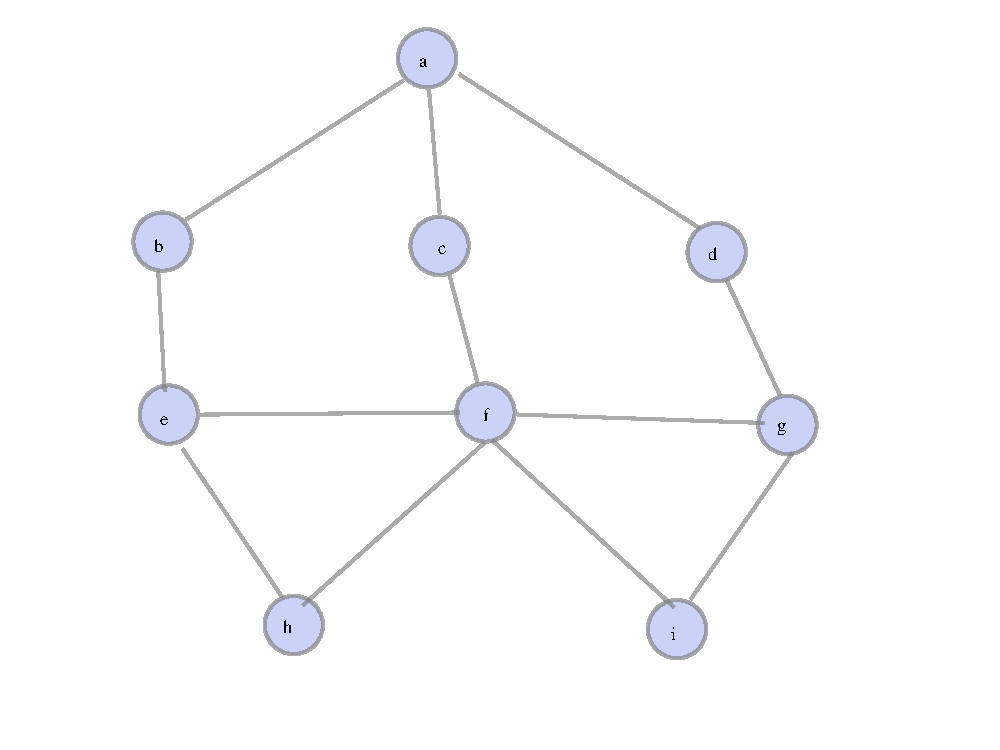
\includegraphics[width=0.8\textwidth]{BN_mrlzd.pdf}
  \caption{Moralized Graph}
\end{figure}
\subsection*{c}
See fig 3
\begin{figure}[H]
  \centering
  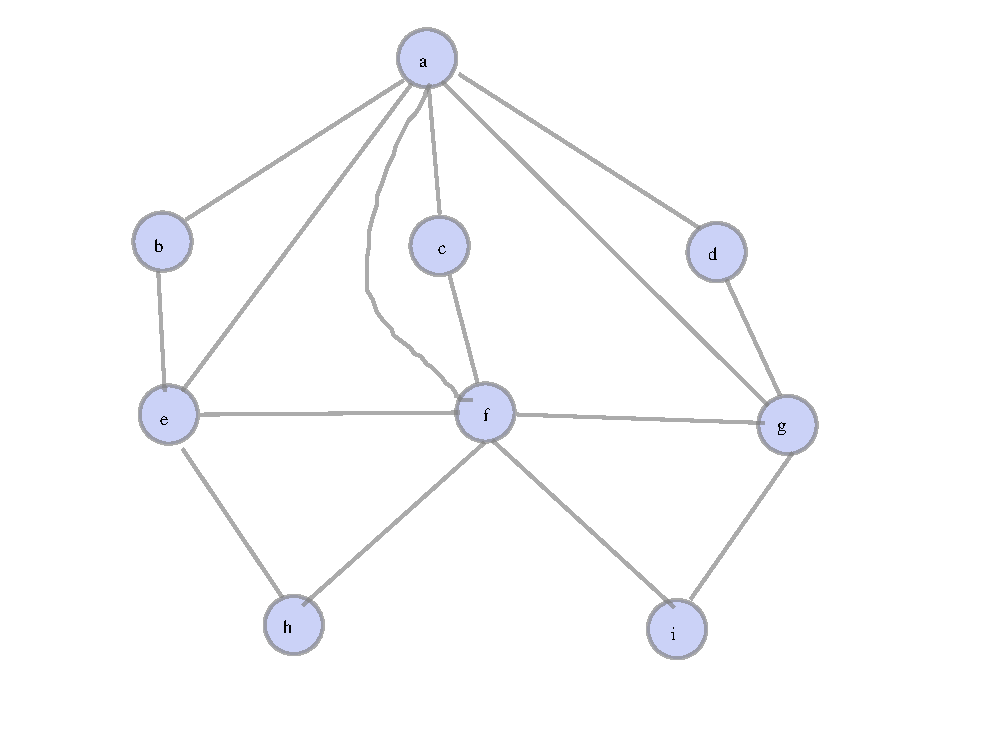
\includegraphics[width=0.8\textwidth]{BN_Trg.pdf}
  \caption{Triangulated Graph}
\end{figure}
\subsection*{d}
See fig 4
\begin{figure}[H]
  \centering
  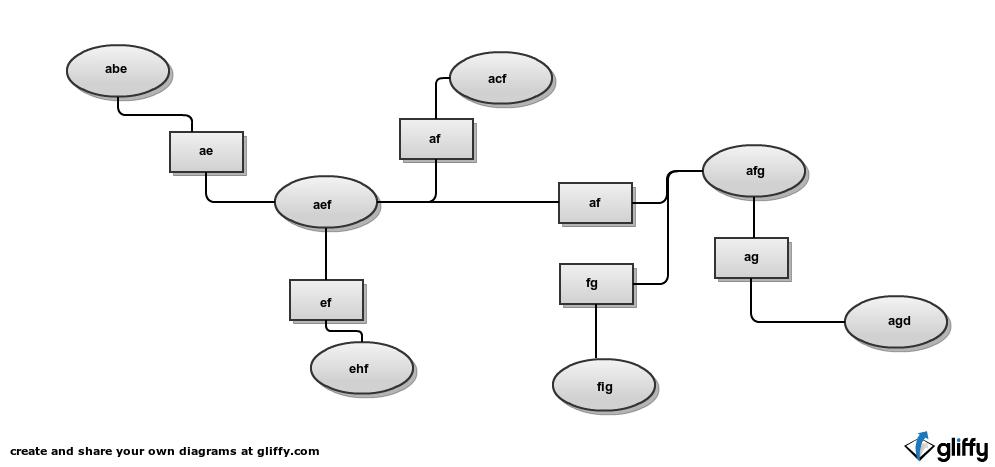
\includegraphics[width=1.1\textwidth]{Juncion_tree.jpg}
  \caption{Junction Tree}
\end{figure}
\subsection*{e}
$\Phi(abe)=p(a)p(b|a)p(e|b)$\\
\indent$\Phi(aef)=1$\\
\indent$\Phi(acf)=p(c|a)p(f|c)$\\
\indent$\Phi(afg)=1$\\
\indent$\Phi(agd)=p(d|a)p(g|d)$\\
\indent$\Phi(ehf)=p(h|e,f)$\\
\indent$\Phi(fig)=p(i|f,g)$\\
and all potentials of separators are set to be 1.

\subsection*{f}
\begin{enumerate}
\item $abe\rightarrow aef:~\Phi^*(ae)= \sum_b\Phi(abe) = p(a)\sum_bp(b|a)p(e|b)$
\item $ehf\rightarrow aef:~\Phi^*(ef)= \sum_h\Phi(ehf) = \sum_hp(h|e,f) = 1$
\item $acf\rightarrow aef:~\Phi^*(af)= \sum_c\Phi(acf) = \sum_cp(c|a)p(f|c)$
\item $\Phi^*(aef)=\Phi(aef)\frac{\Phi^*(ae)\Phi^*(ef)\Phi^*(af)}{\Phi(ae)\Phi(ef)\Phi(af)}$
\item $agd\rightarrow afg:~\Phi^*(ag)= \sum_d\Phi(agd)=\sum_dp(d|a)p(g|d)$
\item $fig\rightarrow afg:~\Phi^*(fg)= \sum_i\Phi(fig)=\sum_ip(i|f,g)=1$
\item $\Phi^*(afg)=\Phi(afg)\frac{\Phi^*(ag)\Phi^*(fg)}{\Phi(ag)\Phi(fg)}$
\item $afg\rightarrow aef:~\Phi^{**}(af)= \sum_e\Phi^*(afg)$
\item $\Phi^{**}(aef)=\Phi^*(aef)\frac{\Phi^{**}(af)}{\Phi^*(af)}$
\item $abe\leftarrow aef:~\Phi^{**}(ae)= \sum_f\Phi^{**}(aef)$
\item $ehf\leftarrow aef:~\Phi^{**}(ef)= \sum_a\Phi^{**}(aef)$
\item $acf\leftarrow aef:~\Phi^{**}(af)= \sum_e\Phi^{**}(aef)$
\item $\Phi^{**}(abe)=\Phi(abe)\frac{\Phi^{**}(ae)}{\Phi^{*}(ae)}$
\item $\Phi^{**}(ehf)=\Phi(ehf)\frac{\Phi^{**}(ef)}{\Phi^{*}(ef)}$
\item $\Phi^{**}(acf)=\Phi(acf)\frac{\Phi^{**}(af)}{\Phi^{*}(af)}$
\item $aef\rightarrow afg:~\Phi^{**}(afg)=\ldots$
\item $afg\rightarrow agd,afg\rightarrow agd$ I'm tired...

\end{enumerate}

\section*{Question 3}
\subsection*{a}
Since $x_{T+1},x_{T+2},\ldots x_T$ do not matter in this question, I have omitted them.
Bayesian Networks as below:
\begin{figure}[H]
  \centering
  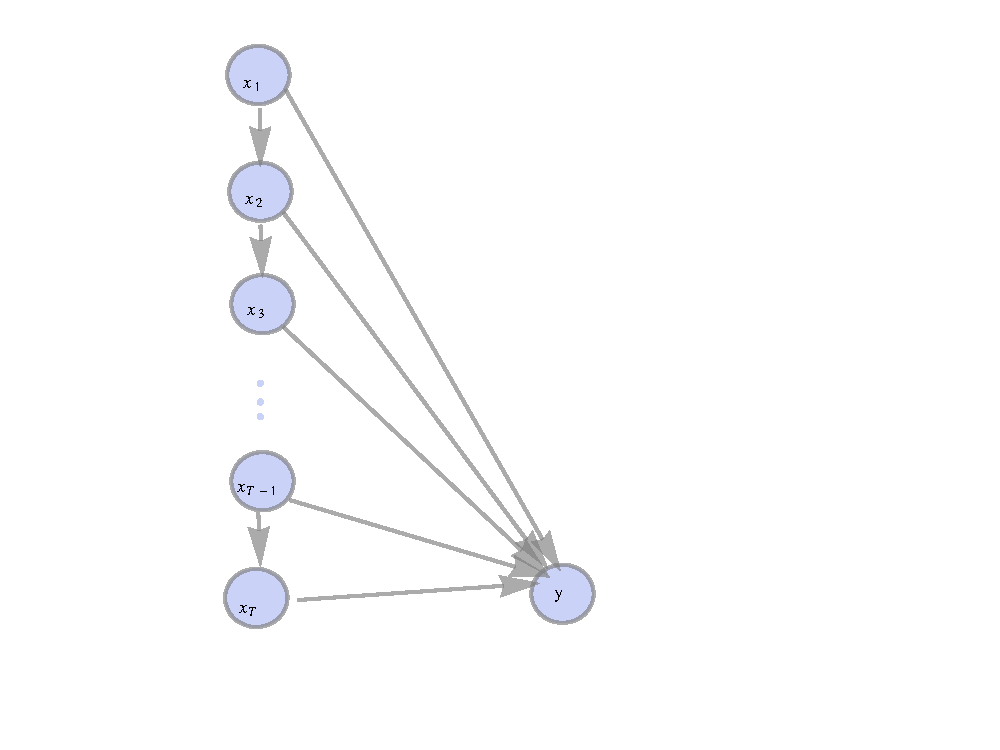
\includegraphics[width=0.8\textwidth]{BN_Q3.pdf}
  \caption{Bayesian Networks}
\end{figure}
Well, the corresponding Junction Tree is pretty complex, I'm not gonna to show a complete figure of it, instead, I would describe it and give a simple illustration when $T=3$.\\
\newline
\textbf{Description:}
\emph{Through the step of \textbf{Moralisation}, since $x_1,x_2,\ldots x_T$ are parents of $y$, all of them should be connected each other. After Moralisation, there is no need to do Triangulation, there are $\left(
\begin{array}{c}
 T+1 \\
 3 \\
\end{array}
\right)$
cliques here, Thus we have 
$\left(
\begin{array}{c}
 T+1 \\
 3 \\
\end{array}
\right)-1$
separators in the\textbf{ Junction Tree}, consider the process of \textbf{Message Passing}, each separator has to be passed twice(two direction), we know that the computation of $P(x_T)$ requires $O(T^3)$ in this case.}\\

Following picture is a Junction Tree when $T=3$,$\left(
\begin{array}{c}
 3+1 \\
 3 \\
\end{array}
\right)=4$ thus we have $4$ cliques.
\begin{figure}[H]
  \centering
  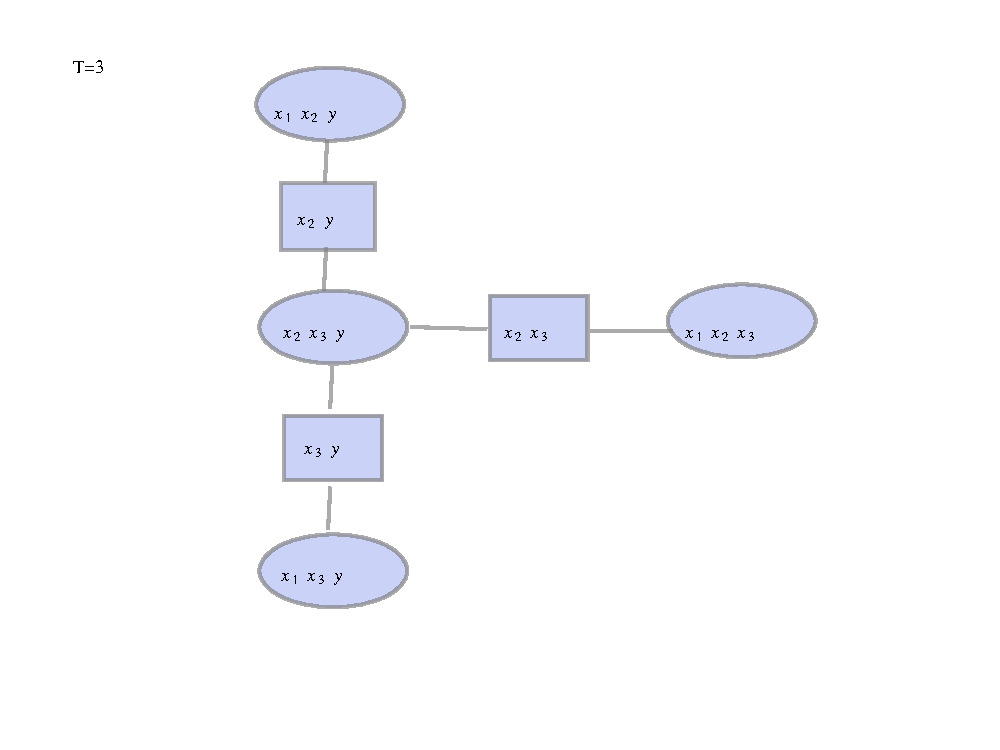
\includegraphics[width=0.8\textwidth]{JT_Q3.pdf}
  \caption{Junction Tree}
\end{figure}

\subsection*{b}
Rewrite the following formula
$$p(x_T)=\sum_{y,x_1,x_2,\ldots,x_{T-1}}p(y|x_1,x_2,\ldots,x_T)p(x_1)\prod_{t=2}^Tp(x_t|x_{t-1})$$
we get
$$p(x_T)=\sum_{y,x_1,x_2,\ldots,x_{T-1}}p(x_1)\prod_{t=2}^Tp(x_t|x_{t-1})\sum_yp(y|x_1,x_2,\ldots,x_T)$$
Note that
$$\sum_yp(y|x_1,x_2,\ldots,x_T)=1$$
we get
$$p(x_T)=\sum_{y,x_1,x_2,\ldots,x_{T-1}}p(x_1)\prod_{t=2}^Tp(x_t|x_{t-1})$$
Which implies
$$p(x_T)=\sum_{x_{T-1}}p(x_T|x_{T-1})p(x_{T-1})$$
We first calculate the table of $p(x_2)$, which requires $O(1)$, then using $p(x_2)$ to calculate the table of $p(x_3)$, which also requires $O(1)$,..., finally we get the result of $p(x_T)$, it's trivial to see that the overall time complexity is $O(T)$.

\section*{Question 4}
\subsection*{a}
run \textbf{SmoothHMM.py} for both evidence sequences, we got:
\begin{enumerate}
\item $e_{1:10} = (F, F, F, T, T, T, T, F, F, F)$\\
   \begin{verbatim}
P(X_1=T|e1:10) = 0.01594
P(X_2=T|e1:10) = 0.02273
P(X_3=T|e1:10) = 0.31481
P(X_4=T|e1:10) = 0.90293
P(X_5=T|e1:10) = 0.94193
P(X_6=T|e1:10) = 0.90294
P(X_7=T|e1:10) = 0.31514
P(X_8=T|e1:10) = 0.02304
P(X_9=T|e1:10) = 0.01736
P(X_10=T|e1:10) = 0.09837
   \end{verbatim}

\item $e_{1:10} = (F, T, F, T, F, T, F, T, F, T)$\\

   \begin{verbatim}
P(X_1=T|e1:10) = 0.24747
P(X_2=T|e1:10) = 0.29091
P(X_3=T|e1:10) = 0.29778
P(X_4=T|e1:10) = 0.29982
P(X_5=T|e1:10) = 0.30030
P(X_6=T|e1:10) = 0.30130
P(X_7=T|e1:10) = 0.30454
P(X_8=T|e1:10) = 0.32356
P(X_9=T|e1:10) = 0.40594
P(X_10=T|e1:10) = 0.71520
   \end{verbatim}
\end{enumerate}

\subsection*{b}
run \textbf{MaxSeq.py}, we got: 
\begin{enumerate}
\item $e_{1:10} = (F, F, F, T, T, T, T, F, F, F)$\\
   \begin{verbatim}
[0, 0, 0, 1, 1, 1, 1, 0, 0, 0]
   \end{verbatim}

\item $e_{1:10} = (F, T, F, T, F, T, F, T, F, T)$\\

   \begin{verbatim}
[0, 1, 0, 1, 0, 1, 0, 1, 0, 1]
   \end{verbatim}
\end{enumerate}
% \section*{Question 2} 
% \begin{figure}[h]
%   \centering
%   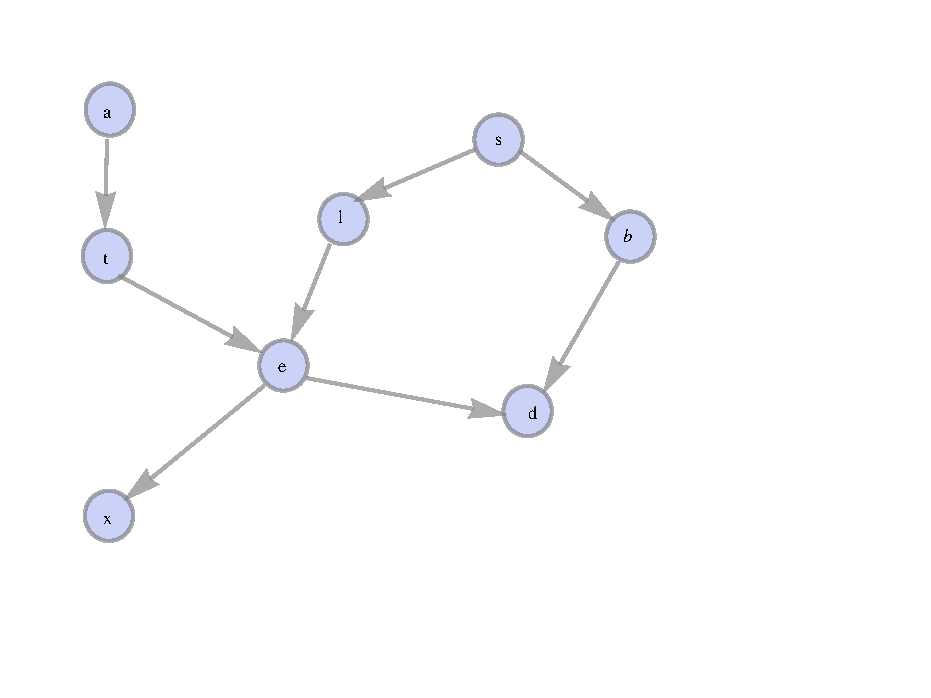
\includegraphics[width=0.8\textwidth]{fig2.pdf}
%   \caption{The Chest Clinic network}
% \end{figure}

% \subsection*{a}
% State if the following conditional independence are true or false:
% \subsubsection*{i} $t\bot s|d$\\
% Use D-separation or D-connection. 
% In the undirected path $t-e-d-b-s-b-s$, $d$ is a collider, thus $t$ and $s$ are D-connected, thus $t\bot s|d$ is false.
% \subsubsection*{ii} $l\bot b|s$\\
% $s$ is not a collider, thus $t\bot s|d$ is true.
% \subsubsection*{iii} $a\bot s|l,d$\\
% There are only two undirected paths from $a$ to $s$, one is  $a-t-e-d-b-s$, all colliders in this path (i.e. $l$) is in $\{l,d\}$, and all non-colliders are not in $\{l,d\}$, thus $a\bot s|l,d$ is false.

% \subsection*{b}
% We use bold font to stand fixed variables, thus
% $P(\mathbf{s}|\mathbf{a},\mathbf{x,b})=\frac{P(\mathbf{s,a,x,b})}{P(\mathbf{a,x,b})}$\\
% $P(\mathbf{s,a,x,b})
% =\sum_{e,t,l}P(\mathbf{s})P(\mathbf{a})P(\mathbf{b|s})P(\mathbf{x}|e)P(e|t,l)P(t|\mathbf{a})P(l|\mathbf{s})
% \\ \indent \indent =P(\mathbf{s})P(\mathbf{a})P(\mathbf{b|s})\sum_{t}P(t|\mathbf{a})
% \sum_{l}P(l|\mathbf{s})
% \sum_{e}P(\mathbf{x}|e)P(e|t,l)$\\
% \\
% $P(\mathbf{a,x,b})
% =\sum_{s,e,t,l}P(\mathbf{a})P(\mathbf{b}|s)P(s)P(\mathbf{x}|e)P(e|t,l)P(t|\mathbf{a})
% \\ \indent \indent =P(\mathbf{a})
% \sum_{s}P(\mathbf{b}|s)P(s)
% \sum_{l}P(l|s)
% \sum_{t}P(t|\mathbf{a})
% \sum_{e}P(\mathbf{x}|e)P(e|t,l)
% $
% \subsection*{c}
% If will know the value of $e$, then the computation complexity would significantly decrease. See the following formulas:\\
% $P(\mathbf{s}|\mathbf{a},\mathbf{x,b,e})=\frac{P(\mathbf{s,a,x,b,e})}{P(\mathbf{a,x,b,e})}$\\
% \\
% $P(\mathbf{s,a,x,b})
% =\sum_{e,t,l}P(\mathbf{s})P(\mathbf{a})P(\mathbf{b|s})P(\mathbf{x}|e)P(e|t,l)P(t|\mathbf{a})P(l|\mathbf{s})
% \\ \indent \indent =P(\mathbf{s})P(\mathbf{a})P(\mathbf{b|s})P(\mathbf{x}|\mathbf{e})
% \sum_{t}P(t|\mathbf{a})
% \sum_{l}P(l|\mathbf{s})
% P(\mathbf{e}|t,l)$\\
% \\
% $P(\mathbf{a,x,b})
% =\sum_{s,e,t,l}P(\mathbf{a})P(\mathbf{b}|s)P(s)P(\mathbf{x}|e)P(e|t,l)P(t|\mathbf{a})
% \\ \indent \indent =P(\mathbf{a})P(\mathbf{x|e})
% \sum_{s}P(\mathbf{b}|s)P(s)
% \sum_{l}P(l|s)
% \sum_{t}P(t|\mathbf{a})
% P(\mathbf{e}|t,l)
% $\\
% We no longer need to sum for the variable $e$.

% \section*{Question 3}
% \subsection*{(a)}
% See the Figure 2
% \begin{figure}[h]
%   \centering
%   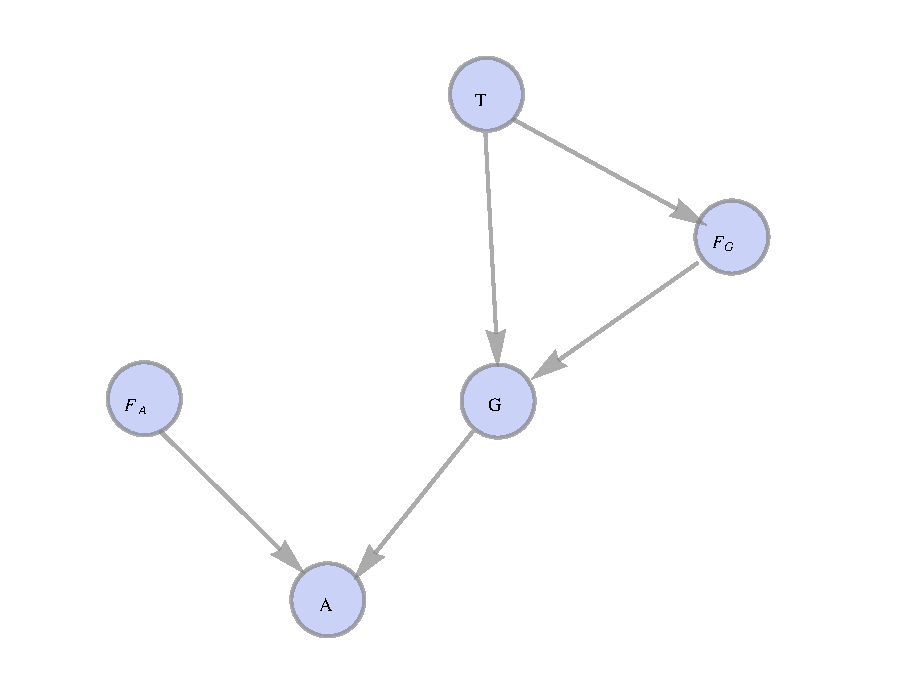
\includegraphics[width=0.7\textwidth]{temp.pdf}
%   \caption{Nuclear Temperature System Network}
% \end{figure}


% \subsection*{(b)}
% See Table 1.
% \begin{table}[h]
% \centering
% \caption{conditional prob table}
%     \begin{tabular}{| c c | c |}
%       \hline
%       $T$  & $F_G$  & $P(G=high|T,F_G)$ \\ \hline
%       high & faulty & $y$\\
%       high & work   & $x$\\
%       normal & faulty & $1-y$\\
%       normal & work   & $1-x$\\
%         \hline
%       \end{tabular}
% \end{table}


% \subsection*{(c)}
% See Table 2.
% \begin{table}[h]
% \centering
% \caption{conditional prob table}
%     \begin{tabular}{| c c | c |}
%       \hline
%       $G$  & $F_A$  & $P(A=sound|G,F_A)$ \\ \hline
%       high & faulty & $0$\\
%       high & work   & $1$\\
%       normal & faulty & $0$\\
%       normal & work   & $0$\\
%         \hline
%       \end{tabular}
% \end{table}

% \subsection*{(d)}
% we have notations: h-high, w-work, s-sound.\\
% $P(T=h|F_A=w,F_G=w,A=s)=\frac{P(T=h,F_A=w,F_G=w,A=s)}{P(F_A=w,F_G=w,A=s)}$, where\\
% $P(T=h,F_A=w,F_G=w,A=s)\\
% \indent \indent = P(T=h)P(F_A=w)P(F_G=w|T=h)\\
% \indent \indent \sum_{G}P(A=s|F_A=w,G)P(G|T=h,F_G=w)$\\
% $P(F_A=w,F_G=w,A=s)\\
% \indent \indent = P(F_A=w)\sum_{T}P(F_G=w|T)P(T)\sum_{G}P(A=s|F_A=w,G)P(G|T,F_G=w)$\\



% \section*{Question 4}
% \subsection*{(a)}
% \begin{figure}[h]
%   \centering
%   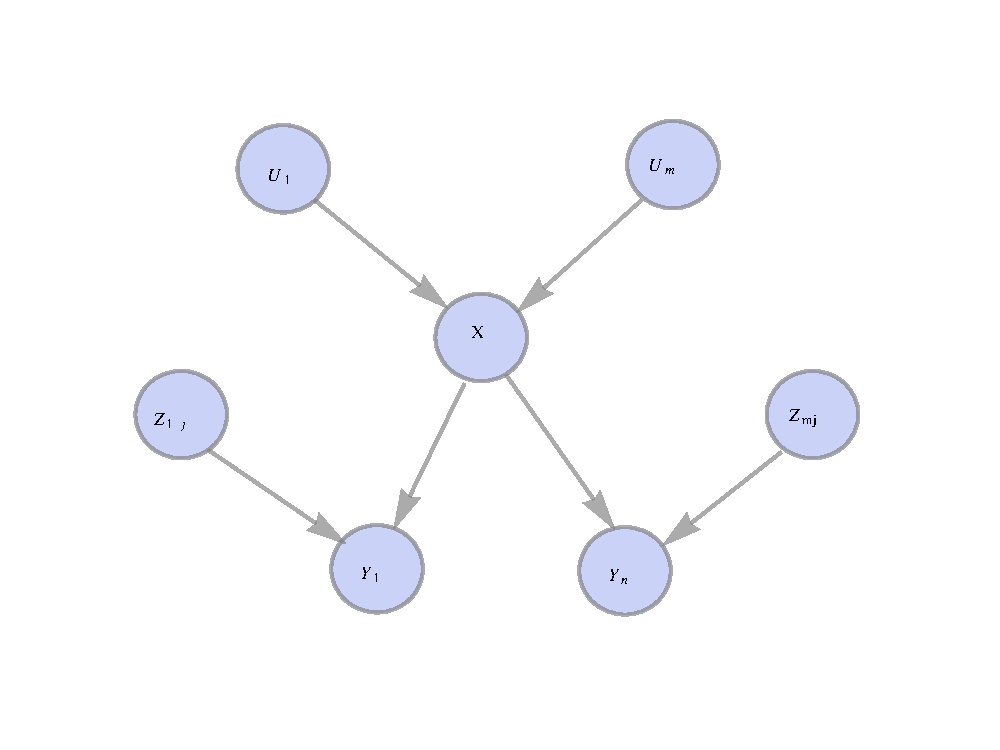
\includegraphics[width=0.7\textwidth]{pic.pdf}
%   \caption{Counterexample}
% \end{figure}

% We prove $P(X|\{U_i\},\{Z_j\})=P(X|\{U_i\})$ by contradiction:\\
% Assume $X$ and $\{Z_i\}$ are D-connected by $\{U_i\}$, then there exist $Z\in\{Z_i\}$
% such that there is a undirected path $U$ from $Z$ to $X$, and all its colliders are in $\{U_i\}$.\\
% \begin{enumerate}
% \item[{\textbf{case 1}}] $U\bigcap \{U_i\}=A\neq\emptyset$\\
% Since every node in $A$ is also in $\{U_i\}$, thus they are all non-colliders, in this case, 
% $X$ and $\{Z_i\}$ are D-connected by the path $U$.

% \item[{\textbf{case 2}}] $U\bigcap \{U_i\}=\emptyset$\\
% Thus $U\bigcap \{Y_i\}=A\neq\emptyset$, from the graph, if there is no collider in $A$, then 
% all arrows in $U$ are in the same direction (either from $Z\leftarrow X$ or $X\leftarrow Z$), but that's not true based on the graph in the question. So, there is at least one collider in $U$, but it is not in $\{U_i\}$, which contradicts to the assumption \textbf{“there exist $Z\in\{Z_i\}$
% such that there is a undirected path $U$ from $Z$ to $X$, and all its colliders are in $\{U_i\}$.”}
% \end{enumerate}
% We therefore have proved that $P(X|\{U_i\},\{Z_j\})=P(X|\{U_i\})$
% \subsection*{(b)}
% $P(X|\{U_i\},\{Y_j\},\{Z_j\})=P(X|\{U_i\},\{Y_j\})$ is no longer true, consider the following
% counterexample (see Figure 3):
% % insert graph
% \begin{figure}[h]
%   \centering
%   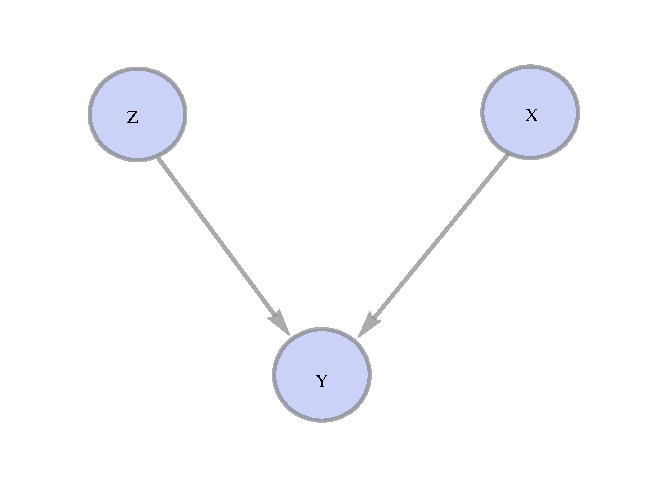
\includegraphics[width=0.5\textwidth]{ct_example.pdf}
%   \caption{Counterexample}
% \end{figure}

% In this case, $\{U_j\}=\emptyset$,$Y$ is a collider, thus $Z$ and $X$ are not conditional independent given $Y$.


\end{document} 



